\section{Resolución de problemas del parcial}
\begin{enumerate}
    \item PIB vs. PNB
        \begin{itemize}
            \item PIB: es restrictivo al territorio.
            \item PNB: palabra clave \textbf{residencia.}
        \end{itemize}
    \item Enfermedad holandesa y el tipo de cambio:
        \begin{itemize}
            \item La moneda local se aprecia.
        \end{itemize}
\end{enumerate}

%%%%%%%%%%%%%%%%%%%%%%%%%%%%%%%%%%%%%%%%%%%%%%%%%%%%%%%%%%%%%%%%%%%%%%%%%%%%%%%%%%%%%%%%%%%%%%%%
\section{Noticia }
\begin{enumerate}
    \item La deuda nacional de EEUU.
    \item EEUU invierte mucho en el asunto de la fuerza militar.
\end{enumerate}

%%%%%%%%%%%%%%%%%%%%%%%%%%%%%%%%%%%%%%%%%%%%%%%%%%%%%%%%%%%%%%%%%%%%%%%%%%%%%%%%%%%%%%%%%%%%%%%%
\section{Discusión de la noticia}
\begin{enumerate}
    \item OTAN 
    \item Trump alega que el resto de europa gasta los bienes comunales, \emph{Citación:``teneis que gastar más para que gasteis menos"}
    \item \textbf{Nos preguntamos:} ¿El sector público va a gastar en un barco o en un hospital, si gasto en el barco la gente que construye el barco lo puede gastar en un horpital, podria decirse que el dinero invertido en el barco va a terminar parcialmente en el hospital? \emph{\textbf{La respuesta a esta pregunta es: } cuando empleamos un recurso la inversión tiene un costo de oportunidad, los recursos económicos que son muy escasos no se pueden invertir en dos cosas, en los estados el problema es que no se sabe en qué invertir.}
    \item Mecanismo de mercado puede retroalimentación inmediata por medio de los beneficios de la empresarialidad.
    \item La defensa del estado nunca tiene una retroalimentación por que no tiene beneficios de empresarialidad y lo hace con el dinero de los demás.
    \item \emph{\textbf{Interesante:} el gasto militar en el mundo está cayendo, ver el ejemplo de los cañones y la mantequilla. \emph{\textbf{Ejemplo: }Si yo convenzo a la gran mayoría a producir mantequilla conseguimos un pseudo-equilibrio.}}
    \item \emph{\textbf{Interesante:} cuando se desarrolló la bomba atómica los costes militares van para abajo.}
\end{enumerate}

%%%%%%%%%%%%%%%%%%%%%%%%%%%%%%%%%%%%%%%%%%%%%%%%%%%%%%%%%%%%%%%%%%%%%%%%%%%%%%%%%%%%%%%%%%%%%%%%
\section{Discusión de clase}
\begin{enumerate}
    \item El multiplicador monetario:  
        \begin{itemize}
            \item \emph{\textbf{Definición de ``Coheficiente de reserva":} los bancos por ley, tienen que guardar parte de sus fondos obligatoriamente en \textbf{efectivo}}.
            \item \emph{\textbf{Ejemplo: } Q 100 de depósito, el banco debe guardar por ley una cantidad en GT es 14\%, entonces Q 14.}
            \item A esto se le llama un multiplciador monetario: 
                \[
                  \text{\text{Coheficiente de reserva}} = 10\% 
                \]
                \[
                  M_{\text{Multiplicador monetario}} = \frac{1}{01} = 10
                \]
                \[
                  M_{\text{Multiplicador monetario}} = \frac{1}{\text{Coheficiente de reserva}}
                \]

            \item 100 C.R.(10) $\Rightarrow$ 90[presto de los 100 iniciales] C.R.(9) $\Rightarrow$ 91 C.R.(8'1) $\Rightarrow$ 78'9 C.R.()
            \item Cuando el banco central regula un coheficiente de reserva de los bancos y lo impone más alto se aumenta la cantidad de dinero en los individuos y las ganancias de lo bancos serán menores, el banco siempre quiere tener el coheficiente de reserva \textbf{bajo}.
            \item  \begin{tabular}{ | p{7cm} | p{7cm} | }
               \hline
                    Activos & Pasivos  \\
               \hline
                    90 Activos & Depósito 100 \\
                    10 Caja & \\
               \hline
            \end{tabular}
            
            \item \textbf{Nos preguntamos:} ¿qúe pasa con un depósito? 
            \begin{center}
            \begin{tabular}{ | p{7cm} | p{7cm} | }
               \hline
                    100 Caja & Depósitos 100 \\ 
                \hline
            \end{tabular}
            \end{center}    

            \begin{center}
            \begin{tabular}{ | p{7cm} | p{7cm} | }
                \hline
                     90 Activos & Depósitos 190 \\
                     100 Caja &  \\  
                \hline
            \end{tabular}
        \end{center}

            
            \item Mientras más coheficiente de reserva menor la ganancia bancaria.
            % \item Comparar los siguientes bancos A \& B: \newline 
        \end{itemize}
    
    \item La curva de rendimientos:
        \begin{itemize}
            \item Los activos a largo plazo tienen un tipo de interés alto y los activos a corto plazo tienen relativamente poco de interés.
            \item El BanGuat 14'M de coheficiente reserva.
            \item \emph{\textbf{Recordar lo siguiente: }La prima de riesgo, inflación, el asunto es que aumenta el interés por que es difícil de anticipar cosas a largo plazo. }
            \item Curva de rendimiento: 
            \begin{center}
            \begin{figure}[htbp]
                \centering
                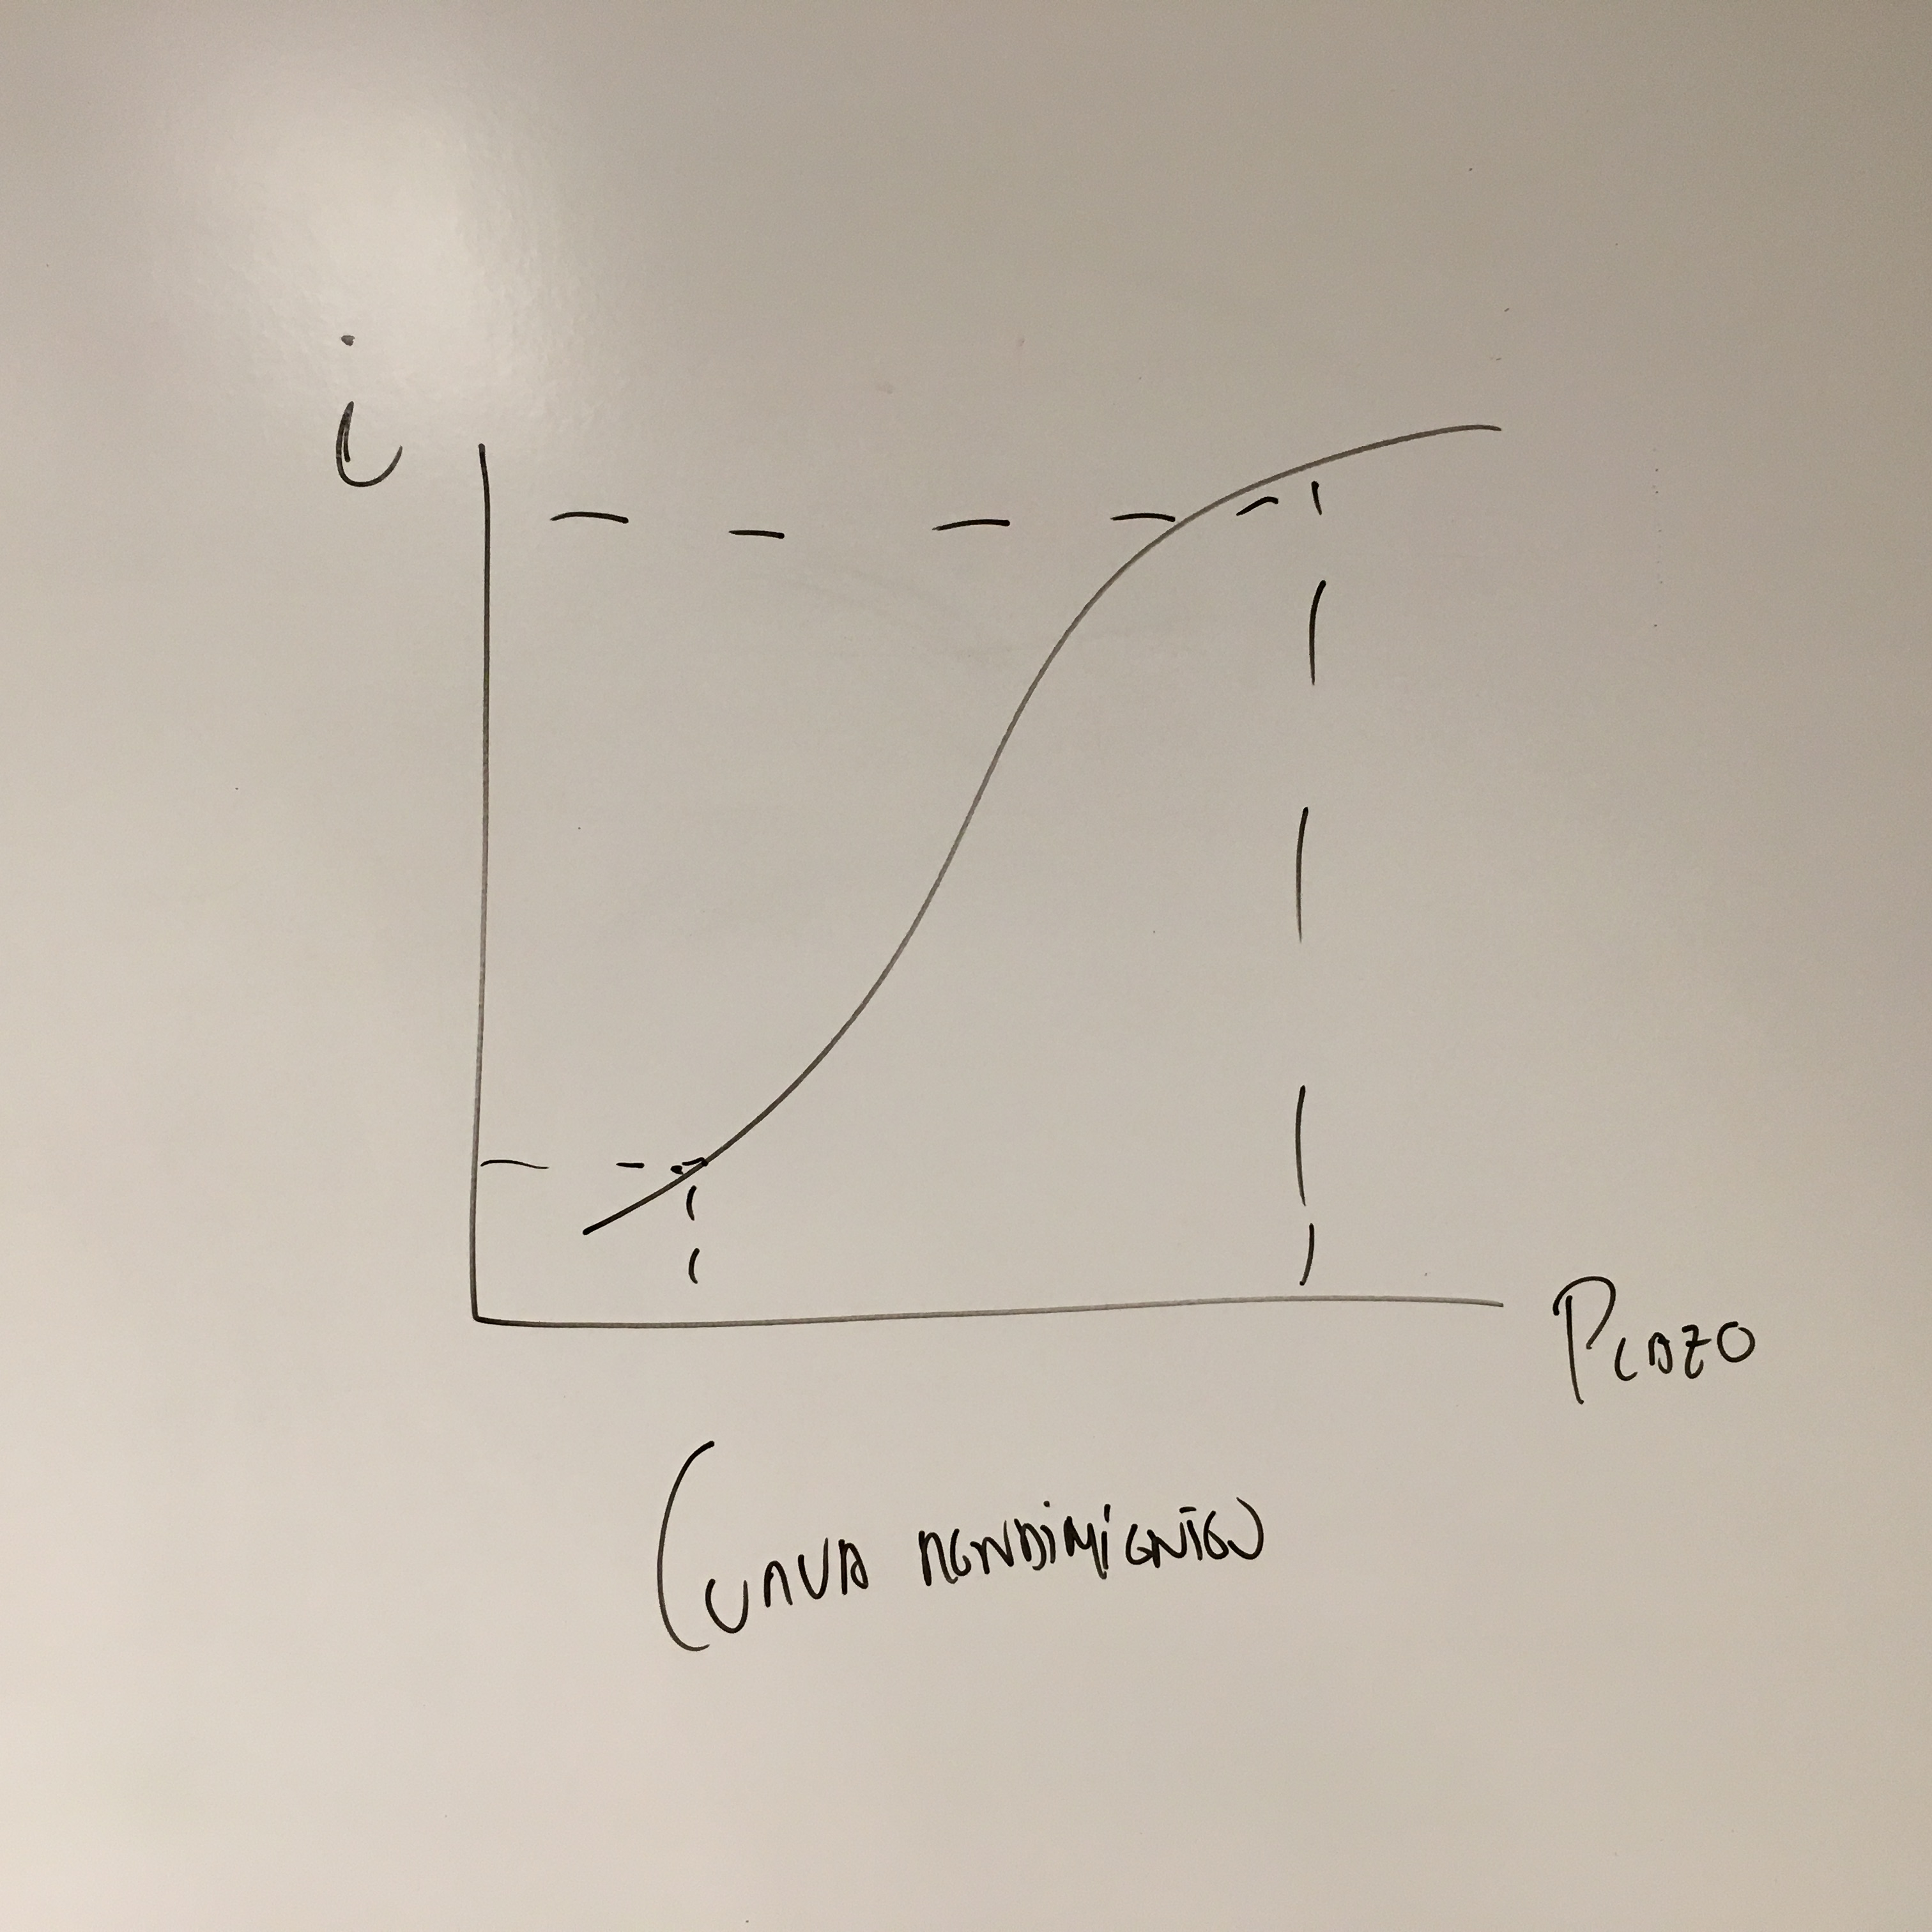
\includegraphics[width=6cm]{Classes/Images/2019-11-04-01.JPG}  
                \caption{}
                \label{}
            \end{figure}              
            \end{center}
        \end{itemize}
    
    \item Banca: comercial y de inversión:
        \begin{itemize}
            \item \emph{\textbf{Definición de ``Comercial":} aquel banco que acepta depósitos del público y da prestamos minoristas a los propios clientes que hacen los depósitos, usualmente prestamos al consumo y prestamos comerciales, hipotecas se consideran prestamos minoristas.}
            \item \emph{\textbf{Definición de ``Inversión":} Leman brothers era un banco de inversión, el banco de inversión no acepta depósitos, y da prestamos mayoritas (usualmente bonos).} \emph{\textbf{Ejemplo: }un banco de inversión le da prestamos a empresas (bonos), el banco de inversión emite deuda,  }
        \end{itemize}
        \begin{center}
        \begin{tabular}{ | p{7cm} | p{7cm} | }
            \hline
            \multicolumn{2}{|c|}{Bancos de inversión} \\
            \hline
                Préstamos (bonos) a empresas  & Deuda de banco (Bonos) \\
            \hline
        \end{tabular}
    \end{center}

    \item Peculiaridades de bancos inversionistas: 
        \begin{itemize}
            \item El banco de inversión: \emph{\textbf{Ejemplo: }ford quiere sacar un nuevo carro, el banco de inversión absorbe la deuda pendiente de ford emitiendo deuda, estos bancos no manejan cuentas individuales.}
            \item Esto pasa mediante bonos.
            \item Esta actividad se llama \emph{dealer} por esto gana interés. Tiene otra actividad que se llama \emph{broker} que básicamente es sentar a los de ford y a la gente que quiere invertir, el banco solo coordina, el banco les cobra a los dos por sentarse en la misma mesa por comisión.  
            \item El banco no es nada más que un comerciante de deudas.
            \item Es la versión bancaria de un fondo de capitales.
            \item \emph{\textbf{Consultar el siguiente recurso:} Fondos del mercado monetario, son casi depositos.}
            \item La banca central no regula estos bancos, a estos los regula otra entidad.
        \end{itemize}
\end{enumerate}



